\documentclass{beamer}
\usepackage{tikz}
\usepackage{amsmath}
\usetheme{Madrid}
\usecolortheme{default}

\title{Flow Control Interfaces in Hardware Design}
\author{}
\date{}

\begin{document}

\frame{\titlepage}

% ============================================================
% SLIDE 1: Valid-Ready Interface (Concept)
% ============================================================
\begin{frame}
\frametitle{Valid--Ready Interface (Concept)}
\framesubtitle{Handshake-Based Protocol}

\begin{itemize}
    \item \textbf{Data transfer} occurs only when both sides agree in the same cycle
    \item \textbf{Sender ready to send data}: \texttt{valid} signal is made 1
    \item \textbf{Consumer ready to receive data}: \texttt{ready} signal is made 1
    \item \textbf{Transfer condition}: if \texttt{(valid == 1 \&\& ready == 1)}, data transfer occurs
\end{itemize}

\vspace{0.3cm}
\textbf{Backpressure Mechanism:}
\begin{itemize}
    \item Flow control where receiver tells sender to slow down or stop
    \item When \texttt{ready = 0} $\rightarrow$ sender must hold
    \item Prevents overflow or data loss
    \item Backpressure is \textbf{explicit}
\end{itemize}

\vspace{0.3cm}
\textbf{Pros:} Simple, no data loss, easy backpressure, widely used, works with FIFOs/pipelines \\
\textbf{Cons:} Throughput depends on handshake, can create combinational loops, higher latency if stalls occur

\end{frame}

% ============================================================
% SLIDE 2: Valid-Ready Interface (Diagram)
% ============================================================
\begin{frame}
\frametitle{Valid--Ready Interface (Diagram)}

\begin{center}
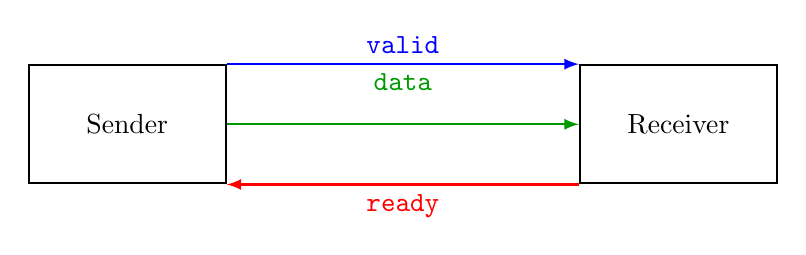
\begin{tikzpicture}[>=latex, thick]
    % Sender box
    \node[draw, rectangle, minimum width=2.5cm, minimum height=1.5cm] (sender) at (0,0) {Sender};
    
    % Receiver box
    \node[draw, rectangle, minimum width=2.5cm, minimum height=1.5cm] (receiver) at (7,0) {Receiver};
    
    % Valid signal (Sender to Receiver)
    \draw[->, blue] (sender.north east) -- node[above] {\texttt{valid}} (receiver.north west);
    
    % Ready signal (Receiver to Sender)
    \draw[<-, red] (sender.south east) -- node[below] {\texttt{ready}} (receiver.south west);
    
    % Data signal
    \draw[->, thick, green!60!black] (sender.east) -- node[above, yshift=0.3cm] {\texttt{data}} (receiver.west);
\end{tikzpicture}
\end{center}

\vspace{0.5cm}
\textbf{Signal Description:}
\begin{itemize}
    \item \texttt{valid}: Asserted by sender when data is ready to be sent
    \item \texttt{ready}: Asserted by receiver when it can accept data
    \item \textbf{Data transfer}: Occurs when \texttt{valid = 1} AND \texttt{ready = 1}
\end{itemize}

\vspace{0.3cm}
\[
\text{Transfer} = \text{valid} \land \text{ready}
\]

\end{frame}

% ============================================================
% SLIDE 3: Valid-Credit Interface (Concept)
% ============================================================
\begin{frame}
\frametitle{Valid--Credit Interface (Concept)}
\framesubtitle{Credit-Based Flow Control}

\begin{itemize}
    \item \textbf{Receiver sends credits} to sender, indicating how much data it can receive in advance
    \item Sender sends data \textbf{as long as it has credits}
    \item \textbf{Credits} represent buffer slots available at the receiver
\end{itemize}

\vspace{0.3cm}
\textbf{Signal Roles:}
\begin{itemize}
    \item \texttt{valid} signal: Data is being sent (from sender)
    \item \texttt{credit} signal: Buffer slots available (from receiver)
    \item Receiver makes \texttt{credits = B}: Sender sends for B beats without waiting for ready per cycle
    \item Each cycle: \texttt{credit = credit - 1}
\end{itemize}

\vspace{0.3cm}
\textbf{Transfer Condition:} Data transfers if \texttt{(valid == 1 \&\& credit > 0)}

\vspace{0.3cm}
\textbf{Pros:} Higher throughput, high speed, good for long latency links and interconnects \\
\textbf{Cons:} More complex logic, needs buffers/FIFOs, overflow risk if mismanaged

\end{frame}

% ============================================================
% SLIDE 4: Valid-Credit Interface (Diagram)
% ============================================================
\begin{frame}
\frametitle{Valid--Credit Interface (Diagram)}

\begin{center}
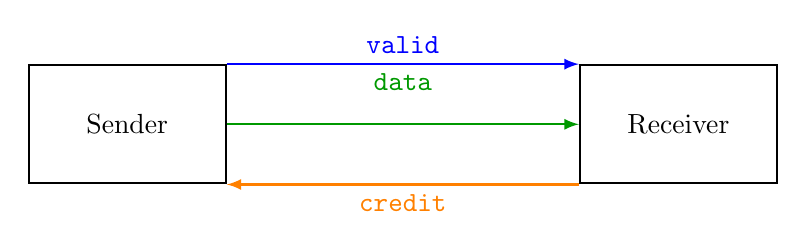
\begin{tikzpicture}[>=latex, thick]
    % Sender box
    \node[draw, rectangle, minimum width=2.5cm, minimum height=1.5cm] (sender) at (0,0) {Sender};
    
    % Receiver box
    \node[draw, rectangle, minimum width=2.5cm, minimum height=1.5cm] (receiver) at (7,0) {Receiver};
    
    % Valid signal (Sender to Receiver)
    \draw[->, blue] (sender.north east) -- node[above] {\texttt{valid}} (receiver.north west);
    
    % Credit signal (Receiver to Sender)
    \draw[<-, orange] (sender.south east) -- node[below] {\texttt{credit}} (receiver.south west);
    
    % Data signal
    \draw[->, thick, green!60!black] (sender.east) -- node[above, yshift=0.3cm] {\texttt{data}} (receiver.west);
\end{tikzpicture}
\end{center}

\vspace{0.5cm}
\textbf{Signal Description:}
\begin{itemize}
    \item \texttt{valid}: Asserted by sender when data is being transmitted
    \item \texttt{credit}: Sent by receiver to indicate available buffer space
    \item \textbf{Credit decrement}: Each data beat decrements the credit counter
\end{itemize}

\vspace{0.3cm}
\textbf{Credit Mechanism:}
\[
\text{Transfer} = \text{valid} \land (\text{credit} > 0)
\]

\begin{itemize}
    \item Sender tracks credits locally
    \item For each transmission: \texttt{credit = credit - 1}
    \item Receiver periodically sends new credits to replenish
\end{itemize}

\end{frame}

\end{document}
